\documentclass[12pt]{article}
\usepackage[utf8]{inputenc}
\usepackage{amsmath}
\usepackage[T1]{fontenc}


\title{ECE 3413 Lab 04\\*Analysis of Linear Time Invariant (LTI) Systems}
\author{Leomar Dur\'an}
\date{${28}^{\text{th}}$ February 2023}

\usepackage{hyperref}

\usepackage[per-mode=symbol]{siunitx}
\newcommand*\siexpr[2][]{\SI[parse-numbers=false,#1]{#2}}%
\usepackage{xfrac}
\usepackage{amssymb}
\newcommand*\transpose{\mathsf{T}}

\usepackage{mathtools}%
\DeclarePairedDelimiter\brao()%
\DeclarePairedDelimiter\brac[]%
\DeclarePairedDelimiter\braco[)%
\DeclarePairedDelimiter\Brac\{\}%
\DeclarePairedDelimiter\norm\lVert\rVert%
\DeclarePairedDelimiter\piecefn\{.
\DeclarePairedDelimiter\evalat.|

\usepackage{lib/nonfloatenvirons}
\usepackage{booktabs}
\newcommand\ra[1]{\renewcommand*\arraystretch{#1}}
\ra{1.25}
\usepackage{minted}

\usepackage{adjustbox}
\newcommand*\mcadj[7]%
% {#columns}{col spec}{rotation}{adjust spec}
% {before rotated text}{rotated text}{after rotated text}
{%
    \multicolumn{#1}{#2}{%
        \rlap{%
            #5\adjustbox{rotate=#3,#4}{#6}~#7%
        }%
    }%
}

\usepackage{pdfpages}
\usepackage{standalone}
\usepackage{matlab}

\usepackage[skip=\baselineskip,indent=0pt]{parskip}
\setlength\parindent{0pt}

\def\hr{{\par\noindent\rule{\textwidth}{0.4pt}}}

\begin{document}

\maketitle
\newpage

\section{Introduction}

The purpose of this experiment is to apply the concept of transfer functions to a translational mechanical system.

The principles used in electrical engineering are shared with other disciplines of engineering.
We can apply these principles to help us look at everyday problems such as a translational system differently,
or we can use this familiarity to better understand the effect of a transfer function in a control system.

This lab also introduces a new type of transfer function, the state-space model which is represented by the \mintinline{matlab}{ss} class in Matlab.

\section{Procedure}

\subsection{Part 01}

\subsubsection{Step 01 - The simulation}

\paragraph{The Parameters}

In part $1$ we are using standard input functions and applying the transfer function
$$
    G = \frac2{s^2 + 5 s + 9}
$$
to these.

I have written a Matlab script to parameterize the model so that it is more flexible and reusable.
This script is available in Appendix subsection \ref{sap:simulation params}.

It sets up the simulation time \mintinline{matlab}{TSTOP = 10.0} in \si\second, the parameters for the input function and the coefficients and constants for the transfer function.
In Part 01a, this input function is a step function which becomes \mintinline{matlab}{stepFinal = 1} in $\si\volt$ at time \mintinline{matlab}{Tstep = 0}.
In Part 01b, this input function is a ramp function $r(t)$ whose slope becomes $\SI1\volt$ at time \mintinline{matlab}{Tstep = 0} until $r(t) =$ \mintinline{matlab}{stepFinal = 1}.

This script is also reused in Part 02 since it already contains much of the input needed for part 02 (namely, the simulation time and transfer function.

\paragraph{The model}

In Part 01(a), we are modeling a step response. Thus, our input signal is a Heaviside step function as built in Fig. \ref{fig:step response model system}.
The only unique block in this model, the Step block is configured as in Fig. \ref{fig:step response model}.

\begin{figure}[h]
    \centering
    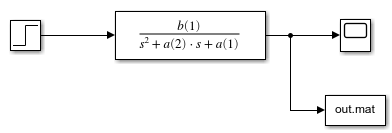
\includegraphics[width=\linewidth]{part01a_step_response_model.png}
    \caption{The system over all for the step response.}
    \label{fig:step response model system}
\end{figure}

\begin{figure}[h]
    \centering
    % 689px = 5in
    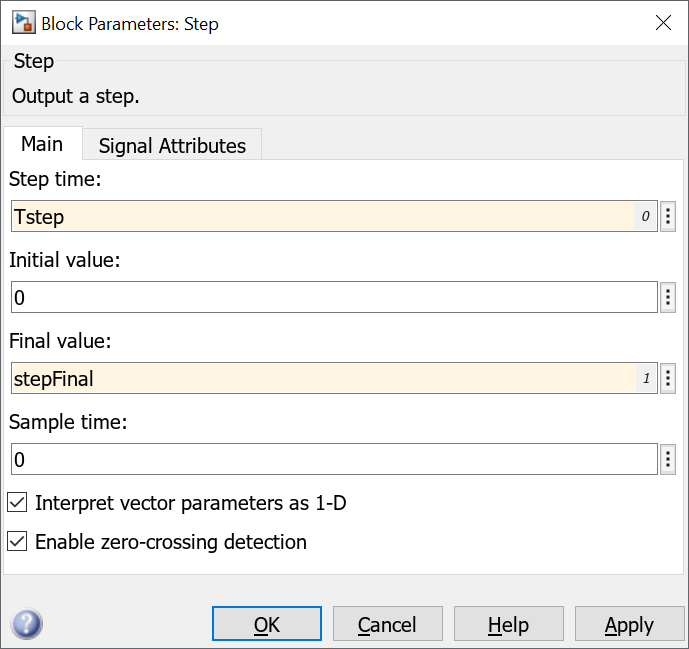
\includegraphics[width=(5in/689)*689]{part01a_step_parameters.png}
    \caption{The configuration for step.}
    \label{fig:step response model}
\end{figure}

\paragraph{Common features}\label{par:common features}

The following features are common to all models simulated in this lab.
All parameters are defined in Appendix subsection \ref{sap:simulation params}.

\begin{figure}[h]
    \centering
    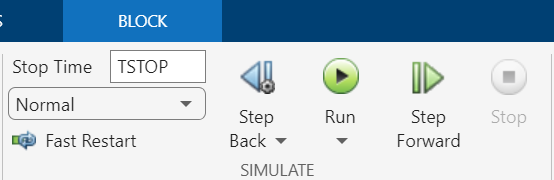
\includegraphics[width=(5in/689)*554]{common_simulation_time.png}
    \caption{The simulation time used in this equation is \mintinline{matlab}{TSTOP}.}
    \label{fig:common simulation time}
\end{figure}

\begin{figure}[h]
    \centering
    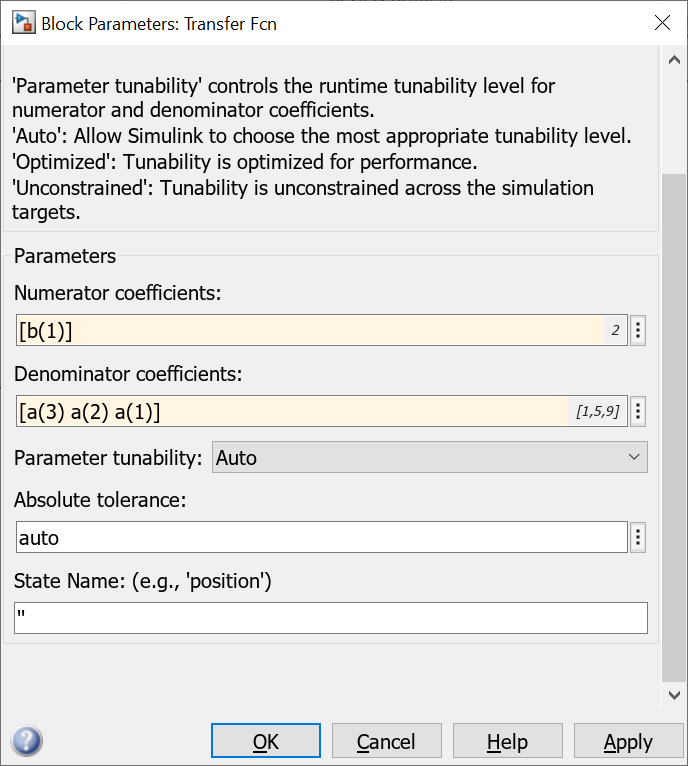
\includegraphics[width=(5in/689)*464]{common_transfer_fcn.png}
    \caption{The transfer function is $\frac{b_1}{s^2 + a_2 s + a_1}$. (Note that Matlab uses $1$-indexed arrays.)}
    \label{fig:common transfer fcn}
\end{figure}

\begin{figure}[h]
    \centering
    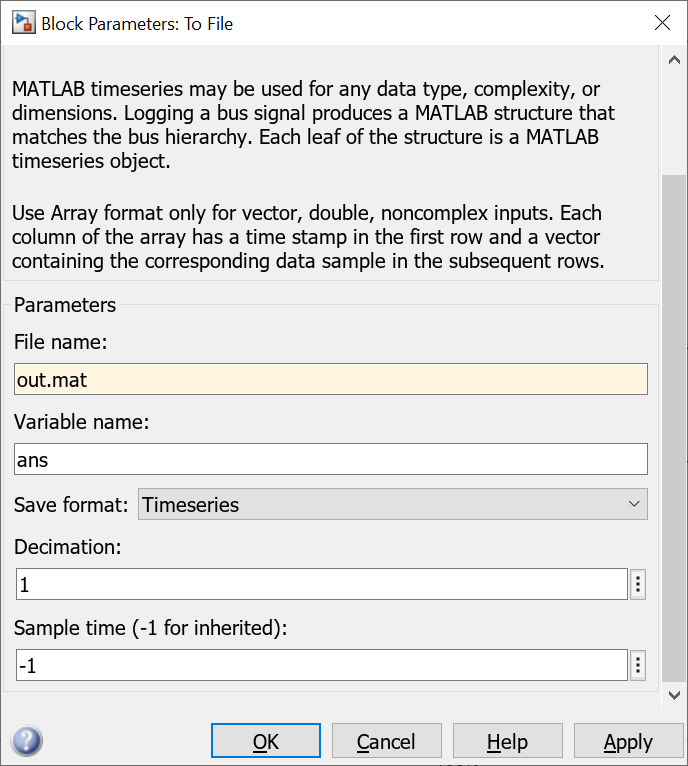
\includegraphics[width=(5in/689)*688]{common_to_file.png}
    \caption{All models will output the timeseries data of the response to the file \mintinline{matlab}{out.mat} to the default variable \mintinline{matlab}{ans}.}
    \label{fig:common to file}
\end{figure}

\begin{enumerate}
    \item
        Given the transfer function
        \begin{equation}
            G_2 = \frac{b}{s^2 + as + b},
        \end{equation}
        
        let the damping ratio and natural frequency, respectively $\zeta, \omega_n \in \mathbb{R}$ s.t. $a = 2\zeta\omega_n$ and $b = \omega_n^2$. So
        \begin{equation}
            \piecefn*{
                \begin{matrix}
                    \omega = \sqrt{b}\rlap, \\*
                    \zeta = \dfrac{a}{2\sqrt{b}}\rlap. \\*
                \end{matrix}
            }\rlap{$\qquad\brao*{b > 0}$}
        \end{equation}

        Furthermore
        \begin{equation}
            \zeta\omega_n = \frac{a}2,
        \end{equation}
        and
        \begin{equation}
            \sqrt{1 - \zeta^2} = \sqrt{1 - \brao*{\sfrac{a}{\brao*{2\sqrt{b}}}}^2} = \frac{1}{2\sqrt{b}} \sqrt{4b - a^2}.%
            \hskip1em\brao*{a < 2\sqrt{b}}
        \end{equation}
        
        We find that the peak time
        \begin{equation}
            T_p = \frac\pi{\omega_n \sqrt{1 - \zeta^2}} = \frac\pi{\brao*{\sqrt{b}}\brao*{ \frac{1}{2\sqrt{b}}\sqrt{4b - a^2}}} = \frac{2\pi}{\sqrt{4b - a^2}}.
        \end{equation}

        We find that the overshoot rate
        \begin{equation}
            \begin{array}{*2{@{}r}@{}l@{}}
                \% OS
                &{}:={}& \exp\brao*{\dfrac{-\zeta\pi}{\sqrt{1 - \zeta^2}}} \SI{100}\percent
            \\*[1.3em]
                &{}={}& \exp\brao*{-\zeta\omega_n\brao*{\dfrac{\pi}{\omega_n\sqrt{1 - \zeta^2}}}} \SI{100}\percent
            \\*
                &{}={}& \exp\brao*{-\brao*{\zeta\omega_n}^{\vphantom{1}}T_p} \SI{100}\percent
            \\*
                &{}={}& \exp\brao*{-\brao*{\tfrac{a}2}^{\vphantom{1}}T_p} \SI{100}\percent
            \\*
                & {}={} & \exp\brao*{\dfrac{-aT_p}{2}} \SI{100}\percent\rlap.
            \\*
            \end{array}
        \end{equation}

        We find that the settling time
        \begin{equation}
            T_s \approx \frac4{\zeta\omega_n} = \frac4{\brao*{\sfrac{a}2}} = \frac8a.
        \end{equation}

        Finally, we find that the rise time
        \begin{equation}
            T_r = 
        \end{equation}

        Let's evaluate at $a = 4, b = 25$. Well $b = 25 > 0$ and $a = 4 < 10 = 2\sqrt{b}$.
        The peak time
        \begin{equation}
            T_p = \frac{2\pi}{\sqrt{4\brao{25} - \brao4^2}} = \siexpr{0.6\overline956}\second.
        \end{equation}
        The overshoot rate
        \begin{equation}
                \% OS
                ={} \exp\brao*{\frac{-\brao4\brao{\SI{0.6856}\second}}2} \SI{100}\percent = \siexpr{2\overline5.38}\percent.
        \end{equation}
        The setting time
        \begin{equation}
            T_s \approx \frac84 = \SI2\second.
        \end{equation}

\end{enumerate}

\subsection{A translational mechanical system}

A state-space representation is a mathematical model of a physical system using variables that are in the time domain.

We are given the translational mechanical system
%in Fig. \ref{fig:translational mechanical system}
that outputs $x_3\brao*t$.
From this system, let's define masses
\begin{equation}
    \vec{M} := \brac*{
        \begin{matrix} M_1 & M_2 & M_3 \end{matrix}
    }^\transpose = \brac*{
        \begin{matrix} \SI1{\kilo\gram} & \SI1{\kilo\gram} & \SI1{\kilo\gram} \end{matrix}
    }^\transpose\rlap,
\end{equation}
spring constants
\begin{equation}
    \vec{K} := \brac*{
        \begin{matrix} K_1 & K_2 \end{matrix}
    }^\transpose = \brac*{
        \begin{matrix} \SI1{\newton\per\meter} & \SI1{\newton\per\meter} \end{matrix}
    }^\transpose\rlap,
\end{equation}
and damping constants
\begin{equation}
    \vec{D} := \brac*{
        \begin{matrix} D_1 & D_2 \end{matrix}
    }^\transpose = \brac*{
        \begin{matrix} \SI1{\newton\second\per\meter} & \SI1{\newton\second\per\meter} \end{matrix}
    }^\transpose\rlap.
\end{equation}

\subsubsection{Free body diagram}
This system has the free body diagram shown in the CAD drawing on the following page.
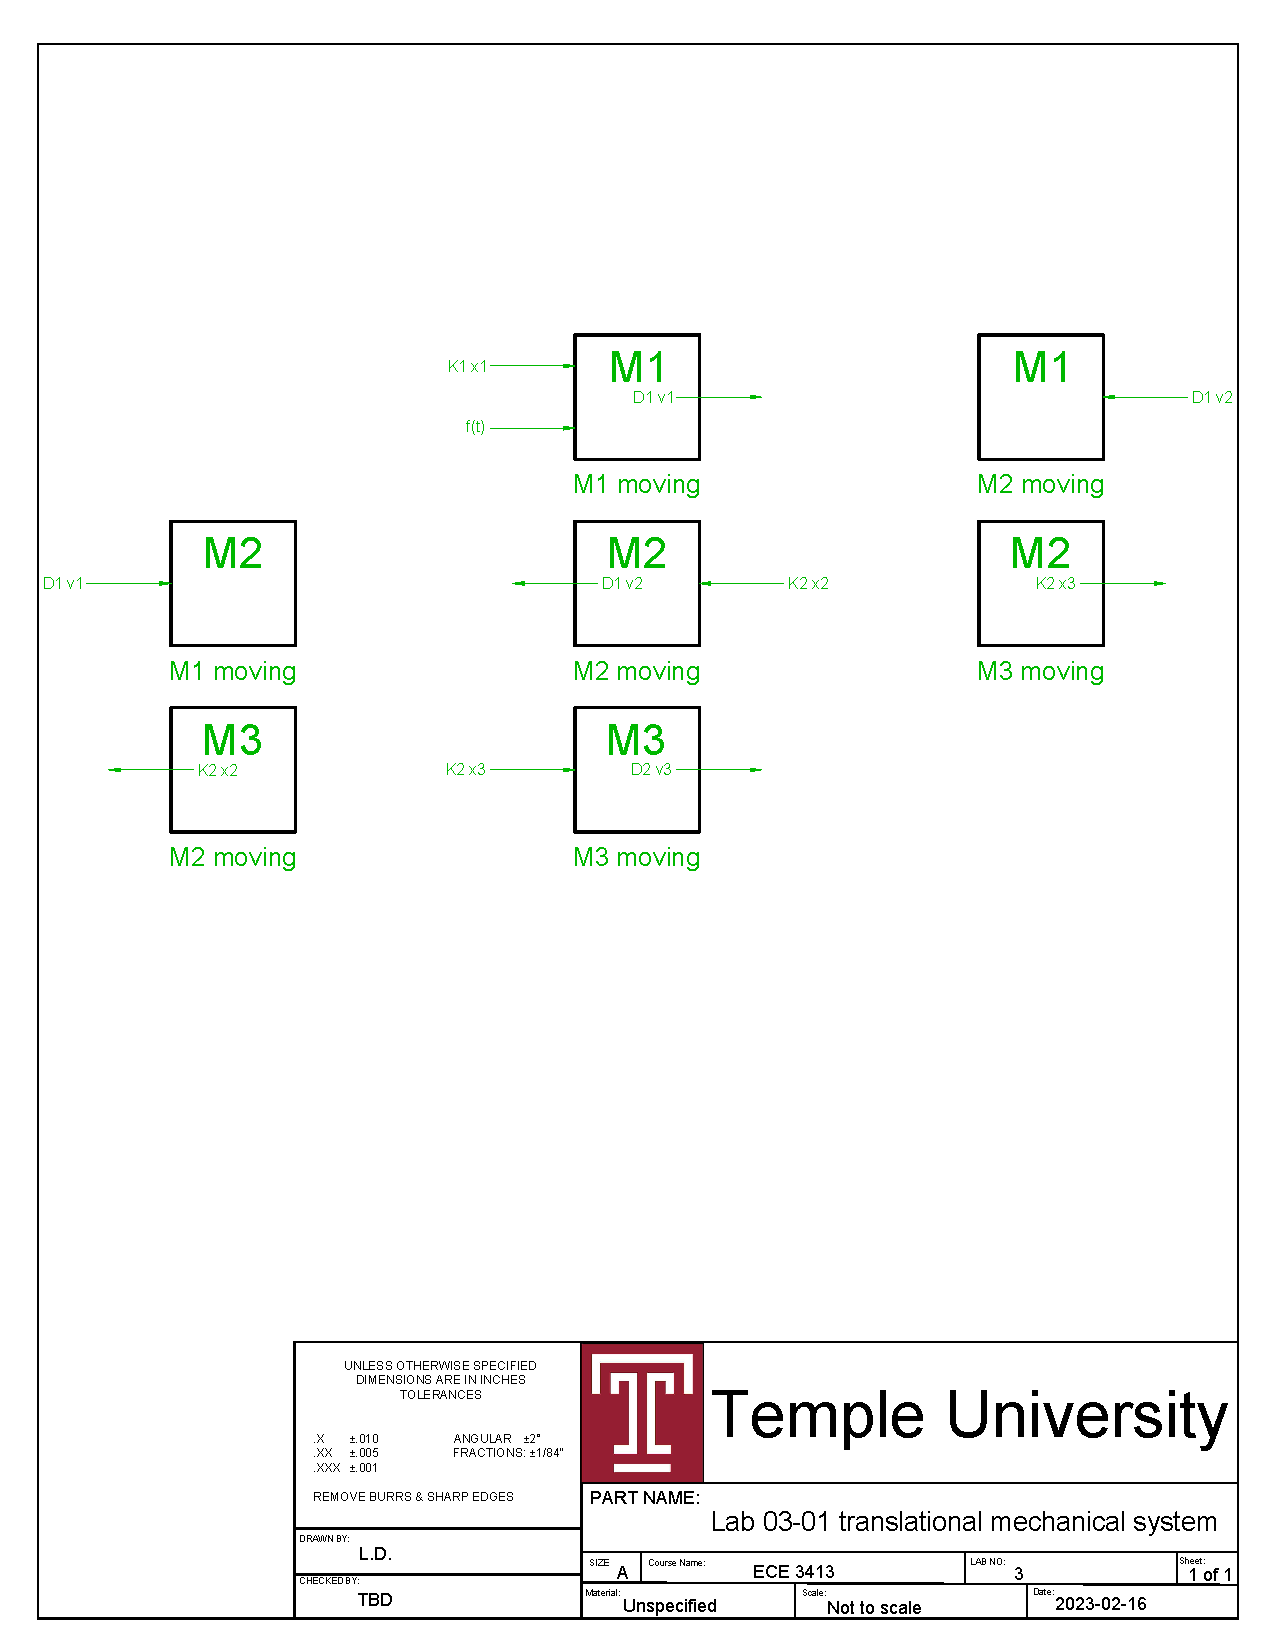
\includepdf{lab03-01 translational mechanical system fbd-A size.pdf}

\subsubsection{Mathematical state-space representation}

Then we find the total force at each mass applying superposition for each possible state.

\begin{equation}
    \piecefn*{
        \begin{array}{@{}l@{}}
            M_1 \ddot{x}_1 = \sum F_{M1\mathrm{x}} = K_1 x_1 + f\brao*t + D_1 \brao*{\dot{x}_1 - \dot{x}_2}\rlap,
        \\*
            M_2 \ddot{x}_2 = \sum F_{M2\mathrm{x}} = D_1\brao*{\dot{x}_1 - \dot{x}_2} + K_2\brao*{-x_2 + x_3}\rlap,
        \\*
            M_3 \ddot{x}_3 = \sum F_{M3\mathrm{x}} = K_2\brao*{-x_2 + x_3} + D_2\dot{x}_3\rlap.
        \\*
        \end{array}
    }
\end{equation}

Next, we relate states $\underline{\hat{x}} \in \mathbb{R}^6$ to position as in Table \ref{tab:states to position}.

\begin{table}[h]
    \centering
    \caption{How states relate to the position variables}
    \[
        \begin{array}{@{}r@{}c@{}l@{}}
        \toprule
            \text{state} & & \text{position}
        \\*
        \midrule
            {\hat{x}}_1 &{}={}& \dot{x}_1\rlap,
        \\*
            {\hat{x}}_2 &{}={}& x_1\rlap,
        \\*
            {\hat{x}}_3 &{}={}& \dot{x}_2\rlap,
        \\*
            {\hat{x}}_4 &{}={}& x_2\rlap,
        \\*
            {\hat{x}}_5 &{}={}& \dot{x}_3\rlap,
        \\*
            {\hat{x}}_6 &{}={}& x_3\rlap.
        \\*
        \bottomrule
        \end{array}
    \]
    \label{tab:states to position}
\end{table}

Thus, we can the derivatives of the states to the states with
the output $y := x_3 = {\hat{x}}_6$ represented by the first row
and using
the force equations for even rows, representing accelerations,
and the state--position relations for odd rows after the first, representing velocities,
giving the state-space representation

\begin{equation}
    \begin{array}{*4{@{}c}@{}}
            \mcadj1{@{}c@{}}{45}{}{\phantom{$=$}}{$
                = \brac*{
                    \begin{array}{@{}c@{}}
                        y
                    \\*
                    \midrule
                        \dot{\underline{\hat{x}}}
                    \\*
                    \end{array}
                }
            $}{}
        & &
            \mcadj1{@{}c@{}}{45}{}{\phantom{$=$}}{$
                =: \brac*{
                    \begin{array}{@{}c|c@{}}
                             D & \mathbf{C}
                    \\*
                    \midrule
                        \vec{B} & \mathbf{A}
                    \\*
                    \end{array}
                }
            $}{}
        &
            \mcadj1{@{}c@{}}{45}{}{\phantom{$=$}}{$
                = \brac*{
                    \begin{array}{@{}c@{}}
                        f
                    \\*
                    \midrule
                        \underline{\hat{x}}
                    \\*
                    \end{array}
                }
            $}{}
    \\*
        \brac*{
            \begin{array}{@{}c@{}}
                y \\*
            \midrule
                \dot{\hat{x}}_1 \\* \dot{\hat{x}}_2 \\*
                \dot{\hat{x}}_3 \\* \dot{\hat{x}}_4 \\*
                \dot{\hat{x}}_5 \\* \dot{\hat{x}}_6 \\*
            \end{array}
        }
        &{}={}&
        \brac*{
            \begin{array}{@{}c|*6c@{}}
                0 & 0 & 0 & 0 & 0 & 0 & 1
            \\*
            \midrule
                \sfrac1{M_1} & \sfrac{+D_1}{M_1} & \sfrac{K_1}{M_1} & \sfrac{-D_1}{M_1} & 0 & 0 & 0
            \\*
                0 & 1 & 0 & 0 & 0 & 0 & 0
            \\*
                0 & \sfrac{+D_1}{M_2} & 0 & \sfrac{-D_1}{M_2} & \sfrac{-K_2}{M_2} & 0 & \sfrac{+K_2}{M_2}
            \\*
                0 & 0 & 0 & 1 & 0 & 0 & 0
            \\*
                0 & 0 & 0 & 0 & \sfrac{-K_2}{M_3} &  \sfrac{D_2}{M_3} & \sfrac{+K_2}{M_3}
            \\*
                0 & 0 & 0 & 0 & 0 & 1 & 0
            \\*
            \end{array}
        }
        &
        \brac*{
            \begin{array}{@{}c@{}}
                f \\*
            \midrule
                {\hat{x}}_1 \\* {\hat{x}}_2 \\*
                {\hat{x}}_3 \\* {\hat{x}}_4 \\*
                {\hat{x}}_5 \\* {\hat{x}}_6 \\*
            \end{array}
        }.
    \end{array}
\end{equation}

\subsubsection{State-space representation in Matlab}

We can use the Matlab function \mintinline{matlab}{ss} to create a state-space representation object.
This function accepts the matrices of coefficients $\mathbf{A}$, $\vec{B}$, $\mathbf{C}$ and $D$ and returns a transfer function in state-space representation form.

This is a transfer function, just like the rational of polynomials \mintinline{matlab}{tf} and zero/pole/gain form \mintinline{matlab}{zpk}.
The $3$ types of objects are mutually convertible,
by using the target class's function on any transfer function object.

\subsection{Rational of polynomials form}

\subsubsection{Conversion using Matlab}

As stated in the previous section,
we may use the \mintinline{matlab}{tf} to convert from the state-space representation to the rational of polynomials form
just as we have with the zero/pole/gain form.
This gives us the transfer function
\begin{equation}
    T\brao*s = \brao*{\frac{x_3}{F}}\brao*s.
\end{equation}

\subsubsection{Equation for the transfer function}

Given a translational mechanical system with $m$ masses in movement,
we may find the transfer function using the equation
\begin{equation}
    T\brao*s = \mathbf{C}\brao*{s\mathbf{I}_{\brao*{2m}} - \mathbf{A}}\vec{B}
\end{equation}

We use Matlab to calculate the result and compare it to the converted transfer function.

\section{Results}

\hr

% This LaTeX was auto-generated from MATLAB code.
% To make changes, update the MATLAB code and export to LaTeX again.

\documentclass{article}

\usepackage[utf8]{inputenc}
\usepackage[T1]{fontenc}
\usepackage{lmodern}
\usepackage{graphicx}
\usepackage{color}
\usepackage{hyperref}
\usepackage{amsmath}
\usepackage{amsfonts}
\usepackage{epstopdf}
\usepackage[table]{xcolor}
\usepackage{matlab}

\sloppy
\epstopdfsetup{outdir=./}
\graphicspath{ {./part01_translational_mechanical_system_mlx_images/} }

\begin{document}

\matlabtitle{Part 1 $-$ Translational mechanical system}


\matlabheading{As a state-space model}

\begin{par}
\begin{flushleft}
is represented by the matrices of coefficients
\end{flushleft}
\end{par}

\begin{matlaboutput}
Mssr =
 
  A = 
       x1  x2  x3  x4  x5  x6
   x1   1   1  -1   0   0   0
   x2   1   0   0   0   0   0
   x3   1   0  -1  -1   0   1
   x4   0   0   1   0   0   0
   x5   0   0   0  -1   1   1
   x6   0   0   0   0   1   0
 
  B = 
       u1
   x1   1
   x2   0
   x3   0
   x4   0
   x5   0
   x6   0
 
  C = 
       x1  x2  x3  x4  x5  x6
   y1   0   0   0   0   0   1
 
  D = 
       u1
   y1   0
 
Continuous-time state-space model.
\end{matlaboutput}
\end{document}


\ \hr \\*

% This LaTeX was auto-generated from MATLAB code.
% To make changes, update the MATLAB code and export to LaTeX again.

\documentclass{article}

\usepackage[utf8]{inputenc}
\usepackage[T1]{fontenc}
\usepackage{lmodern}
\usepackage{graphicx}
\usepackage{color}
\usepackage{hyperref}
\usepackage{amsmath}
\usepackage{amsfonts}
\usepackage{epstopdf}
\usepackage[table]{xcolor}
\usepackage{matlab}

\sloppy
\epstopdfsetup{outdir=./}
\graphicspath{ {./part02_ratio_of_polynomials_form_mlx_images/} }

\begin{document}

\matlabtitle{Part 2 $-$ Rational of polynomials form}


\matlabheading{1. Conversion using Matlab}

\begin{par}
\begin{flushleft}
The transfer function from the state-space representation
\end{flushleft}
\end{par}

\begin{matlaboutput}
Mtf =
 
                   -s + 2.768e-16
  -------------------------------------------------
  s^6 - s^5 - s^4 - 2 s^3 + 2 s^2 + 2 s + 2.053e-16
 
Continuous-time transfer function.
\end{matlaboutput}

\matlabheading{2. Equation for transfer functions}

\begin{par}
\begin{flushleft}
create a transfer function that is just s
\end{flushleft}
\end{par}

\begin{matlaboutput}
T =
 
                   -s - 1.371e-16
  -------------------------------------------------
  s^6 - s^5 - s^4 - 2 s^3 + 2 s^2 + 2 s - 2.435e-16
 
Continuous-time transfer function.
\end{matlaboutput}

\matlabheading{Coefficient of determination $R^2$}

\begin{par}
\begin{flushleft}
To compare the transfer functions, let's find the $R^2$ value of all coefficients.
\end{flushleft}
\end{par}


\begin{par}
\begin{flushleft}
Then the R\textasciicircum{}2
\end{flushleft}
\end{par}

\begin{matlaboutput}
R2 = 1.0000
\end{matlaboutput}
\begin{matlaboutput}
shows that the coefficients have a strong correlation
\end{matlaboutput}
\begin{matlaboutput}
and are therefore equivalent.
\end{matlaboutput}
\end{document}


\section{Discussion}

After finding the state-space representation,
this experiment becomes very straightforward.
However, that is the difficult part.

What I remembered to help me finish it is that springs act on displacement into the moving mass and viscous dampers aft on velocity away from the moving mass.
After this, the sum of all forces must equal the acceleration of the mass.
Then setting up the matrix of coefficients is not difficult although I may not have been able to think of coming up with the variables myself.
It's a really clever way of solving this problem.

This experiment shows application not only in electrical engineering, but also mechanical and civil engineering of the concept of a control system.
It's interesting to imagine how many of the concepts that we have learned in electrical engineering may be applied to other engineering disciplines or may have even come from methods in other engineering disciplines.

Often times, it seems that less intuitive techniques may make a problem much easier to solve simply by changing the domain or a basis.
This is the principle behind using the Laplace transform to handle transfer functions more easily.

\newpage
\appendix
\section{Appendix}

\subsection{Step 01 (in parts 01 and 02) -- Simulation parameters, Matlab Script}\label{sap:simulation params}
\inputminted{matlab}{step01_simulation_params.m}

\hr

\subsection{Step 01 (in parts 01 and 02) -- Simulation parameters, Matlab Script}
\inputminted{matlab}{step01_simulation_params.m}

\end{document}
